\documentclass{standalone}
\standaloneconfig{border=2mm 2mm 2mm 2mm}

%maths
\usepackage{mathtools}
\usepackage{amsmath}
\usepackage{amssymb}
\usepackage{amsfonts}

%tikzpicture
\usepackage{tikz}
\usepackage{scalerel}
\usepackage{pict2e}
\usepackage{tkz-euclide}
\usetikzlibrary{calc}
\usetikzlibrary{patterns,arrows.meta}
\usetikzlibrary{shadows}
\usetikzlibrary{external}

%pgfplots
\usepackage{pgfplots}
\pgfplotsset{compat=newest}
\usepgfplotslibrary{statistics}
\usepgfplotslibrary{fillbetween}

%colours
\usepackage{xcolor}

\begin{document}

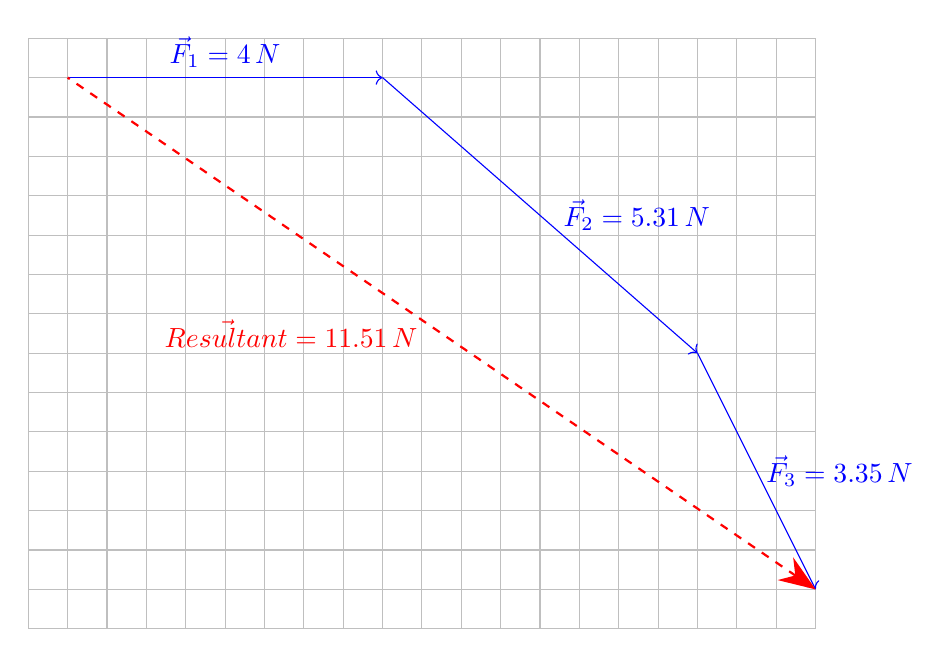
\begin{tikzpicture}
\draw [step=0.5,lightgray] (0,-2.5) grid (10,5);  % Grid
\draw [->, blue] (0.5,4.5) -- (4.5,4.5) node[midway, above] {$\vec{F}_{1} = 4\,N$};
\draw [->, blue] (4.5,4.5) -- (8.5,1) node[midway, right=5pt] {$\vec{F}_{2} = 5.31\,N$};
\draw [->, blue] (8.5,1) -- (10,-2) node[midway, right] {$\vec{F}_{3} = 3.35\,N$};
\draw [{Stealth[scale=2]}-, red, thick, dashed] (10,-2) -- (0.5,4.5) node[midway, left=5pt] {$\vec{Resultant} = 11.51\,N$};
\end{tikzpicture}

\end{document}